\chapter{Prototyping}\label{chp:prototyping}


%===================================================================================================%
\section{Introduction}
%===================================================================================================%

After evaluating different requirements and therefore task and environment characteristics in chapter~\vref{chp:operationalization}, test cases and prototypes to run against the test cases have to be designed. Similar to the environments outlined in the previous chapter, both prototypes for the no-serverless and serverless approach differ in their basic cloud-platform setup, but are as similar as possible on the logic level to avoid any distortion of the results.

To ensure comparability between both prototypes, basic architecture will remain the same for each system. AWS Kinesis Data-Streams\footnote{\url{https://aws.amazon.com/kinesis/data-streams/}} will be used as a Event-Stream provider and only the data-processing approach will differ between those two prototypes. 

In the following, these prototypes will be discussed and their architecture will be outlined in order to provide the reader a comprehensive insight into the systematic research conducted by the author and thevrefore ensure the explicit and reproducible nature of this paper. 



%===================================================================================================%
\section{Event-Stream}\label{chp:protoEvent-Stream}
%===================================================================================================%

To generate the incoming messages, the AWS Kinesis Data Generator Project\footnote{\url{https://github.com/awslabs/amazon-kinesis-data-generator}} is used. The AWS CloudFormation service is used to provision a simple data-generator instance. The template used to to so can be seen in the appendix A on page~\pageref{app:cloudformation}. It is a web client that uses user-supplied parameters to create messages on the data-stream. 

%===================================================================================================%
\section{Non-Serverless}\label{chp:protoNSL}
%===================================================================================================%

The non-serverless prototype utilizes long-running Docker container (which were discussed in chapter~\vref{chp:container}). The the basic system's architecture is outlined in figure~\vref{fig:nslArchitecture}. All of the business logic is contained and run inside docker containers that are deployed in the cloud. They subscribe to the message stream, receive messages and process them accordingly. 

\begin{figure}[ht]
    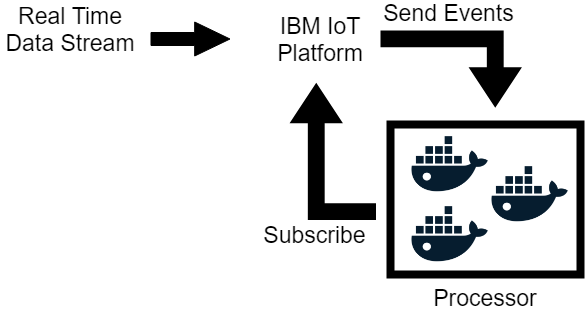
\includegraphics[width=\linewidth]{images/streaming/containerArch.png}\centering
    \caption
    {Non-Serverless Stream Processing Architecture}
    \label{fig:nslArchitecture}
\end{figure}

To subscribe to incoming messages, the official AWS NodeJS client library and the corresponding sample code is used.\footnote{\url{https://github.com/awslabs/amazon-kinesis-client-nodejs}} To avoid any distortion of the measurements by compute operations that are not in scope of this study, the incoming messages will only be converted from Celsius to Fahrenheit and logged to console without being written to a database.\\
For the non-serverless approach, containers running the prototype are deployed on AWS to adequately compare the prices of both solutions, a instance type to run the containers has to be chosen that is theoretically capable of the same compute power a serverless approach can deliver. The following system model is based on approximations and assumptions since non-serverless and serverless compute power is not possible to directly compare.


In chapter~\vref{chp:operationalization}, a test case was designed where 10,000 messages per second are being produced. To calculate the theoretically required non-serverless producers the following formulas\autocite{AmazonFAQs} can be used:

$\textbf{incoming-write-bandwidth-in-KB} = \\
\text{average-data-size-in-KB} * \text{number-of-records-per-seconds}$

$\textbf{outgoing-read-bandwidth-in-KB} = \\
\text{incoming-write-bandwidth-in-KB} * \text{number-of-consumers}$

$\textbf{\# Consumers} = \\
max(\text{incoming-write-bandwidth-in-KB}/1000, \text{outgoing-read-bandwidth-in-KB}/2000)$

Meaning, that either the incoming write bandwidth in Kilobyte divided by 1000 or, the outgoing read bandwidth in Kilobyte divided by 2000 determines the amount of consumers needed depending which of both measurements is higher. The \textit{number-of-consumers} is in this scenario equal to $1$, since the consumer poses as one logical consumer that is scaled horizontally. The \textit{average-data-size-in-KB} is rounded to 1 Kilobyte (see chapter~\vref{fig:messagePayload}), which results in 10 deployed consumer instances. 

Using the official client library\footnote{\url{https://github.com/awslabs/amazon-kinesis-client-nodejs}}, 10 consumer instances have to be deployed to sufficiently process the incoming stream. Utilized are the AWS EC2 C5 instances, which are recommended for this type of workload\footnote{\url{https://aws.amazon.com/ec2/instance-types/}}. For evaluation of processing power, the different types of C5 instances would have to be considered, since they are equipped with different CPU and RAM kits but since this study focuses on general scalability (which is constraint by the architectural pattern and not be the raw compute power for the non-serverless approach) and costs, the cheapest option "C5.large" is used. 


%===================================================================================================%
\section{Serverless}\label{chp:protoSL}
%=======================================================

\begin{figure}[ht]
    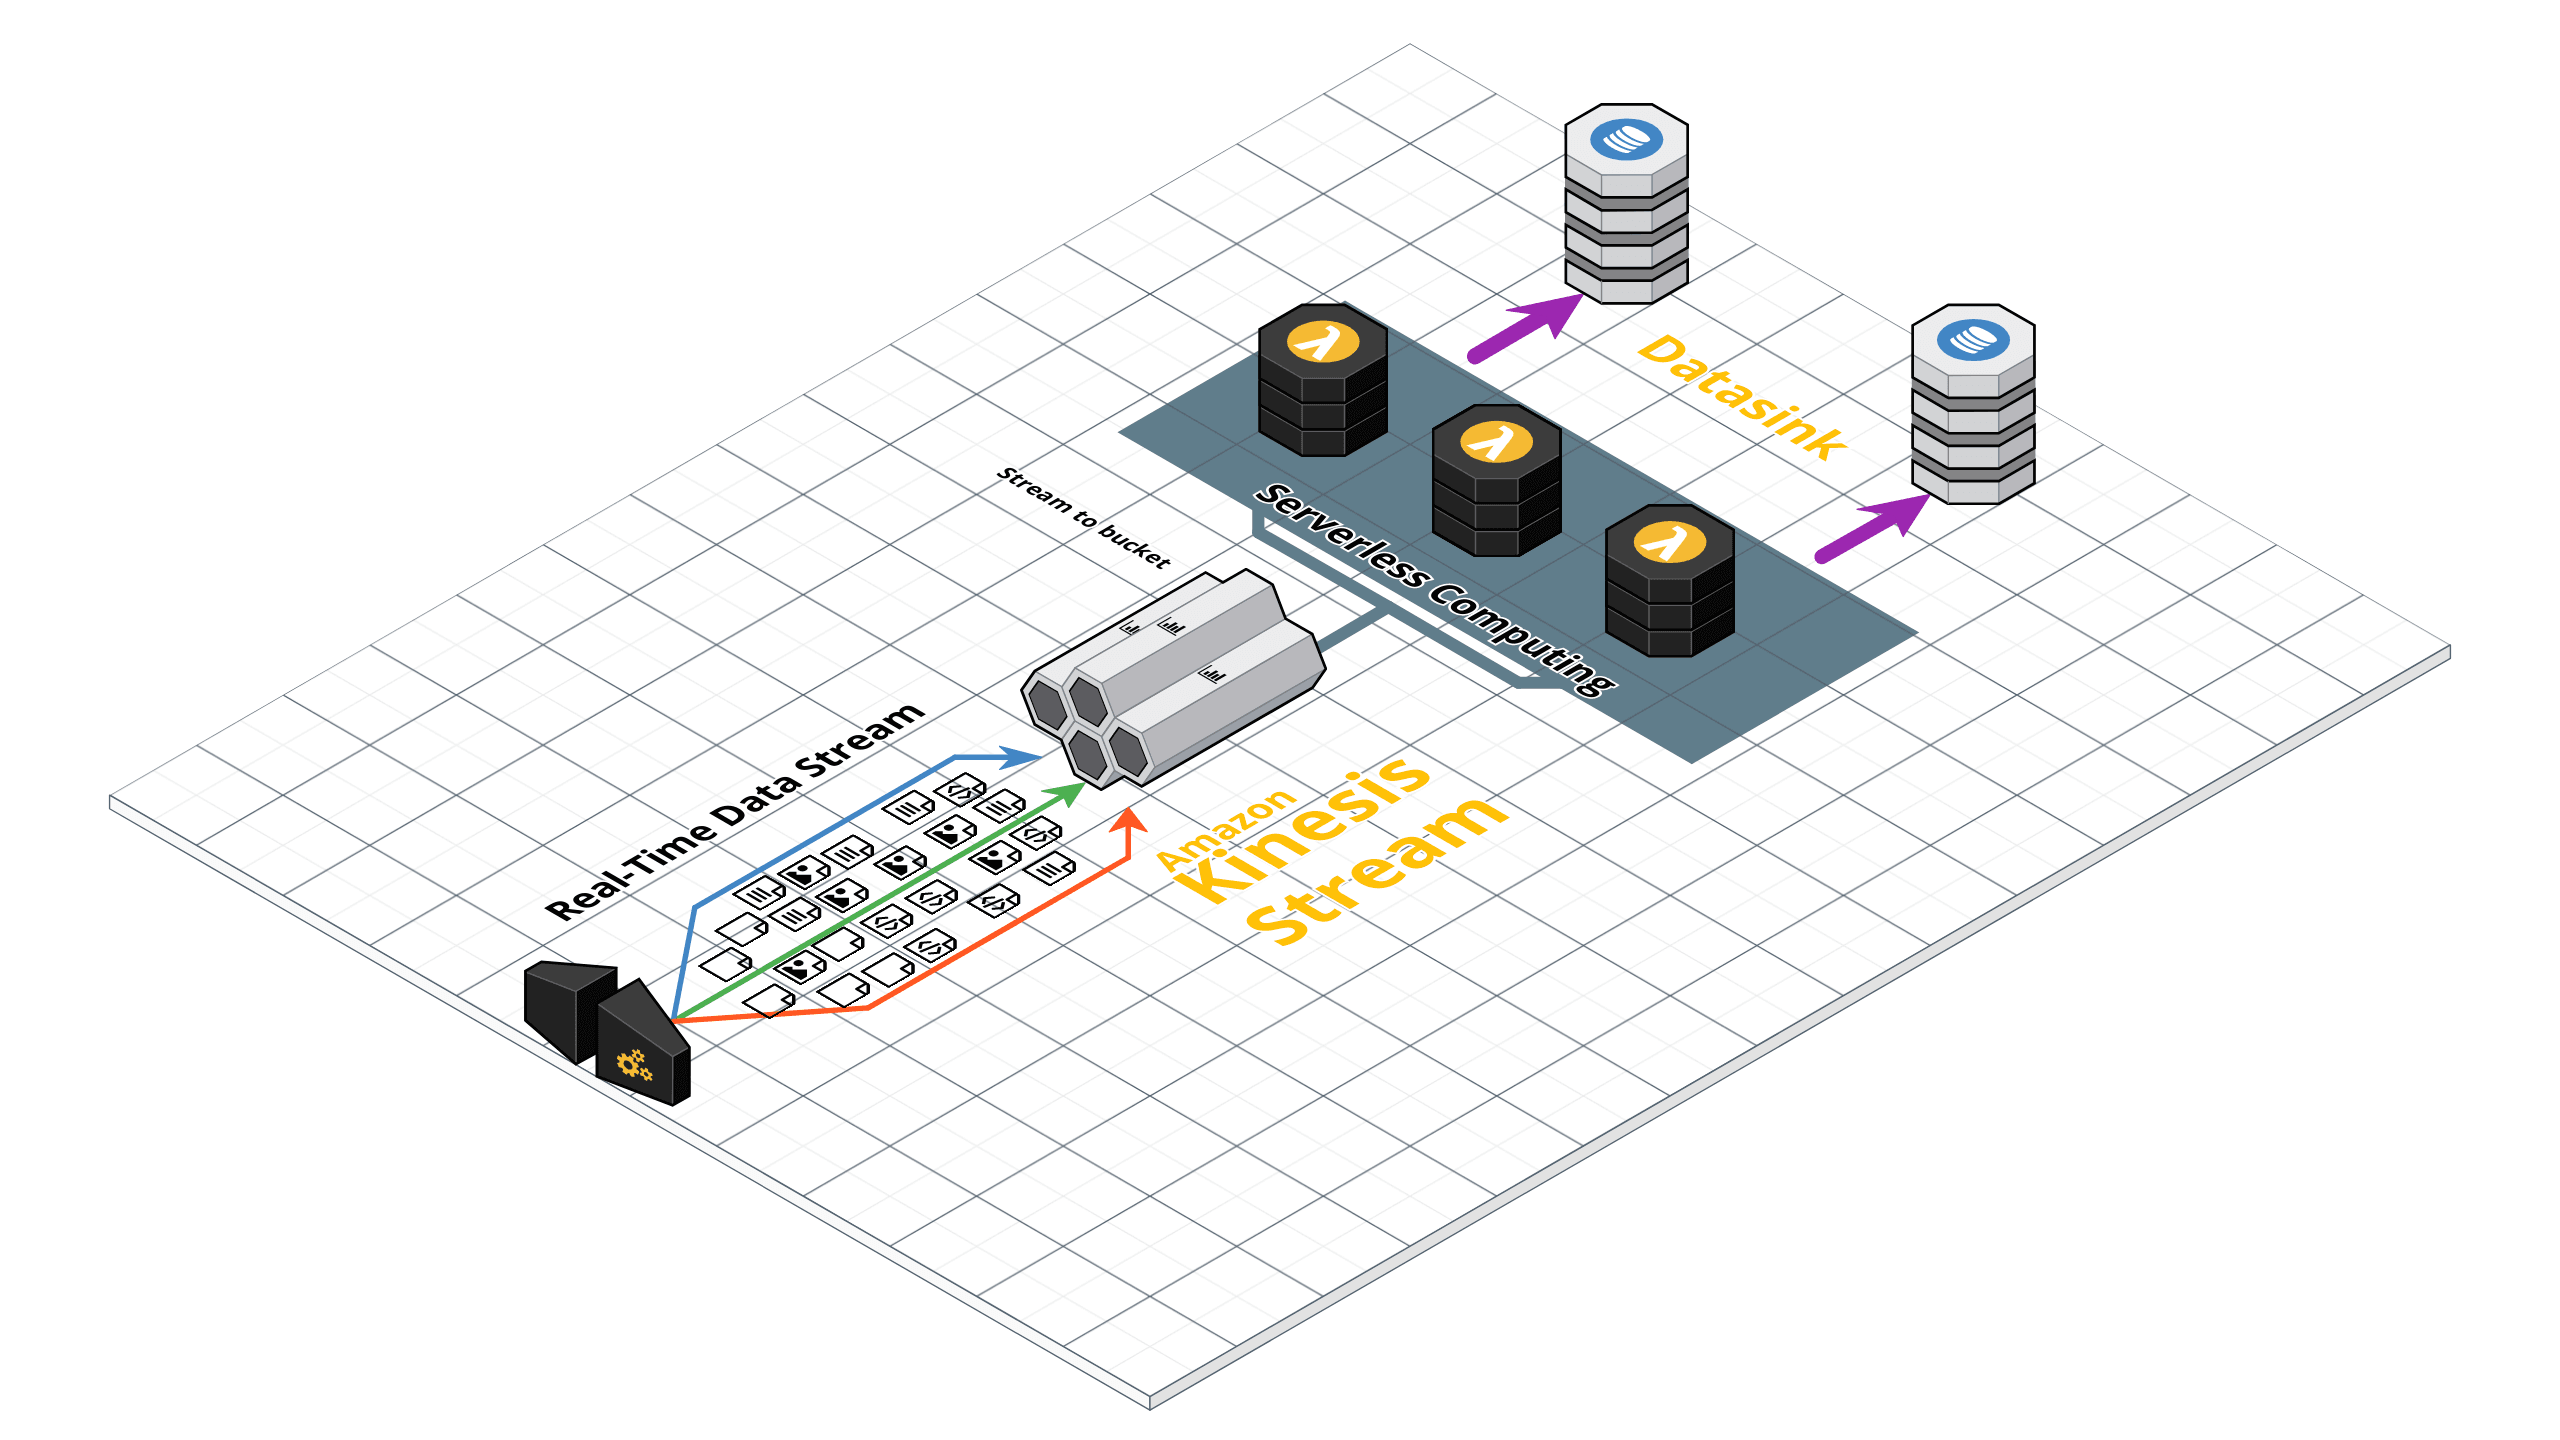
\includegraphics[width=\linewidth]{images/streaming/streamingaws.png}\centering
    \caption
    [AWS Stream Processing Architecture]
    {AWS Stream Processing Architecture}
    \label{fig:awsStreamingArchitecture}
\end{figure}

The serverless compute prototype will be implemented using AWS Lambda. Due to the nature of the service, only the processing logic has to be supplied as code. Provisioning of instances and invocation of functions is entirely done by the platform, thus reducing the amount of work required for a deployment drastically. To execute the logic, an NodeJS 8.10 environment is used and the following code (figure~\vref{code:slProcessor} is deployed:

\begin{figure}[ht]
    \begin{lstlisting}[language=js,firstnumber=1]
    'use strict'
    const AWS = require('aws-sdk')

    /* Unit Conversion */
    const celsiusToFahrenheit = data => {
      const parsedJSON = JSON.parse(
        Buffer.from(data, 'base64').toString('ascii')
      )
      const celsius = parsedJSON.temp
      return celsius * 9 / 5 + 32
    }
    
    exports.handler = (event, context, callback) => {
      /* Process the list of records and transform them */
      const output = event.Records.map(record => ({
        /* This transformation is the "identity" transformation, the data is left intact */
        recordId: record.eventID,
        result: 'Ok',
        data: celsiusToFahrenheit(record.kinesis.data)
      }))
    
      /* Log Results */
      output.map(e => console.log(e.data))
      callback(null, { records: output })
    }
    \end{lstlisting}\centering
    \caption{Code: Serverless Processor}
    \label{code:slProcessor}
\end{figure}

Performance, scaling, invocation and duration metrics are gathered with the AWS Service "CloudWatch", which records the measurements and is not open source. It is assumed that the metrics gathered are correct.


%===================================================================================================%
\section{Summary}
%===================================================================================================%

Using AWS Kinesis as an Event-Stream and AWS Kinesis Data Generator, data ingress (i.e., messages) are generated that will be processed by long-running containers for the non-serverless prototype and AWS Lambda functions that run NodeJS8.10 for the serverless approach.\\
Due to architectural constraints, the number of non-serverless data-consumers is predefined and they have to be manually deployed. For the serverless approach on the other hand, only the processing logic has to be supplied as code. Provisioning of instances and invocation of functions is entirely done by the platform. \\
Recording of measurements is done by the AWS Service "Cloudwatch".